\documentclass[usenames, dvipsnames, no-framenumber]{beamer}

\usepackage[utf8]{inputenc}
\usepackage{xcolor}
\usepackage{cancel}
\usepackage{tikz}
\usetikzlibrary{decorations.pathmorphing,patterns,backgrounds}
\usepackage{multirow}
\usepackage{overpic}



\usefonttheme[onlymath]{serif}


%\usetheme[navigation]{UMONS}
\usetheme[]{UMONS}


\title{Pas si élémentaire\dots~mon cher Watson}
\subtitle{Une enquête au cœur de l'histoire des sciences}
\author[Brandelet, Ducobu, Gamrath]{Antoine Brandelet, Ludovic Ducobu et Sébastien Gamrath}
\date{\vspace{-10ex}}

\institute[]{%
Faculté des Sciences\\
Université de Mons \\
[2ex]
\includegraphics[height=5ex]{UMONS}\hspace{2em}%
\raisebox{-1ex}{\includegraphics[height=10ex]{UMONS_FS}}
\raisebox{-2ex}{
\includegraphics[height=15ex]{images/UMons-Rouge.png}\hspace{2em}}%
\\
\vspace{2ex}
}




\definecolor{vert}{rgb}{0,0.6,0}
\definecolor{rouge}{rgb}{0.7,0,0}


\newcommand{\positif}{\textcolor{OrangeRed}{$\oplus$} }
\newcommand{\negatif}{\textcolor{ForestGreen}{$\ominus$} }



\newcommand{\caneva}[3]{
\draw[color=#3] (-#1/2,-#2/2) -- ++ (0,#2) -- ++ (#1,0) -- ++ (0,-#2) -- cycle;

}

\newcommand{\boule}[2][1]{
  \draw[style={fill=#2}] (0,0) circle(#1);
}

\newcommand{\parachute}{%
\draw[fill=white] (1,0) arc (0:180: 1);
\draw (-1,0)--(1,0);
\draw (0:0)--(30:1);
\draw (0:0)--(60:1);
\draw (0:0)--(90:1);
\draw (0:0)--(120:1);
\draw (0:0)--(150:1);

\draw (1,0)--(0,-1);
\draw (0,0)--(0,-1);
\draw (-1,0)--(0,-1);}

\begin{document}

\begin{frame}[plain]

\maketitle

\end{frame}

\begin{frame}%[plain]
\vspace{1.5cm}
\begin{center}
\itshape
``Lorsque vous avez éliminé l'impossible, ce qui reste, si improbable soit-il, est nécessairement la vérité.''
\end{center}

\begin{flushright}
Sir Arthur Conan Doyle
\end{flushright}

\begin{center}

\includegraphics[scale=.15]{images/Sherlock.jpg}
\end{center}

                
\end{frame}


\begin{frame}%[plain]
\frametitle{Déroulement d'une enquête}

\begin{figure}
\begin{minipage}[c]{.46\linewidth}
\only<1>{\hspace{3em}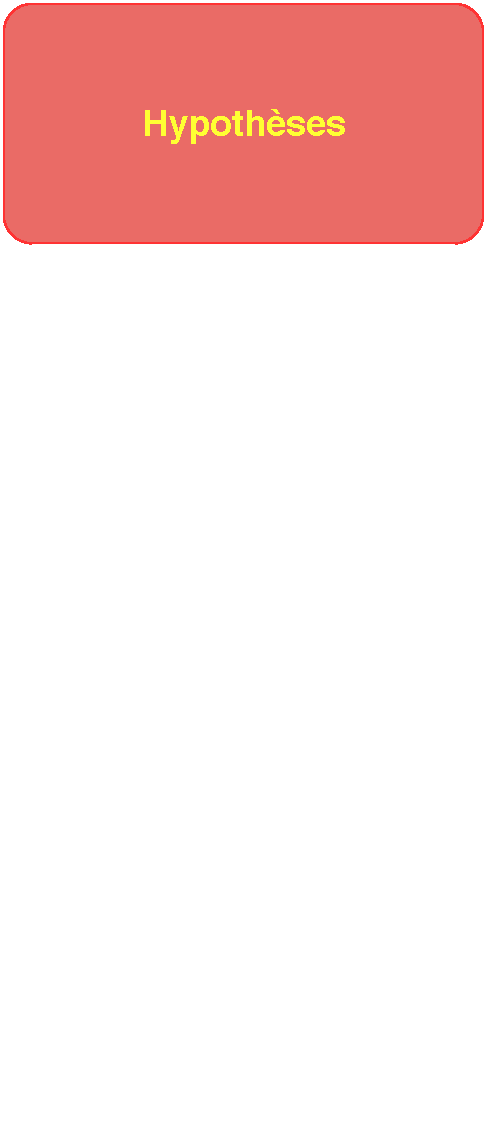
\includegraphics[scale=.4]{images/enth/en1.pdf}}
\only<2>{\hspace{3em}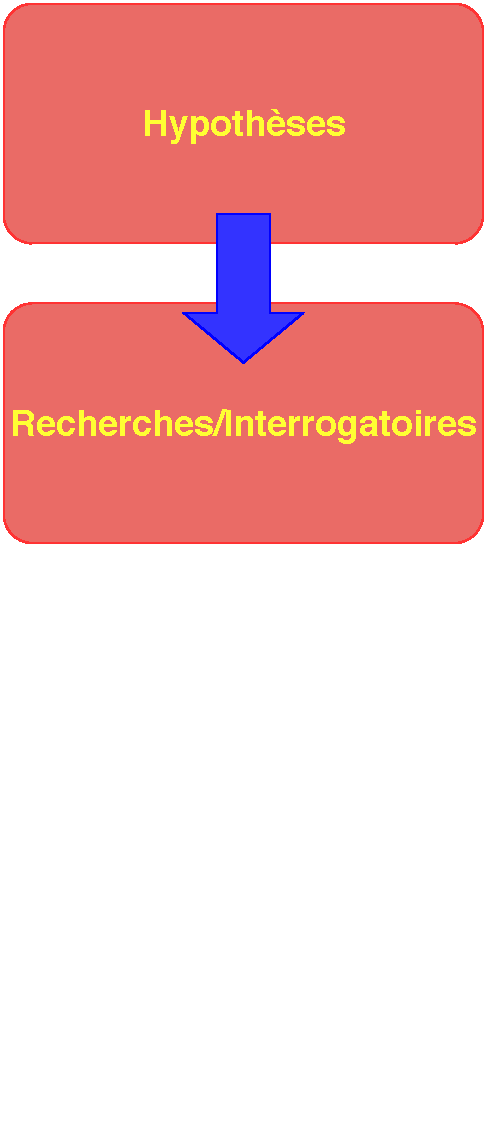
\includegraphics[scale=.4]{images/enth/en2.pdf}}
\only<3>{\hspace{3em}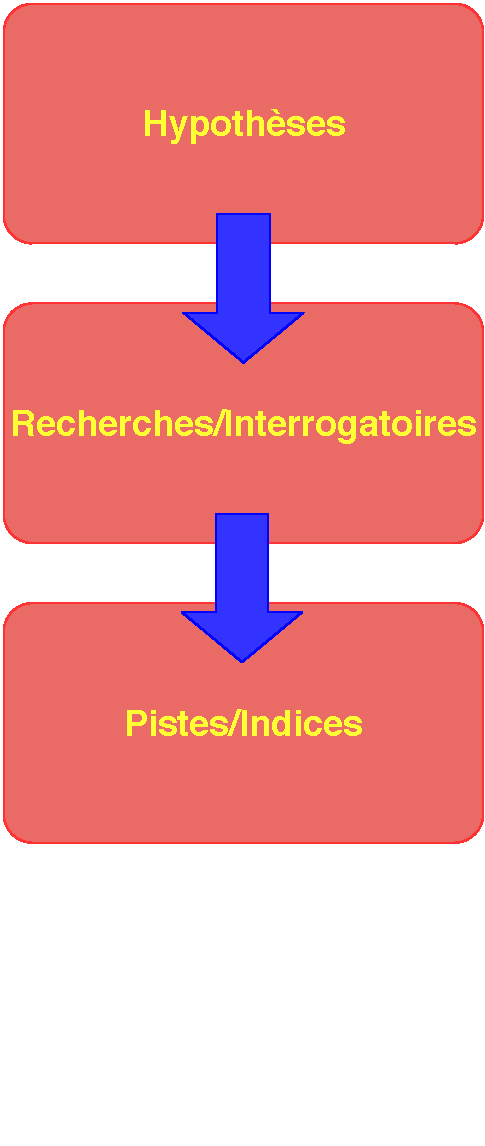
\includegraphics[scale=.4]{images/enth/en3.pdf}}
\only<4>{\hspace{3em}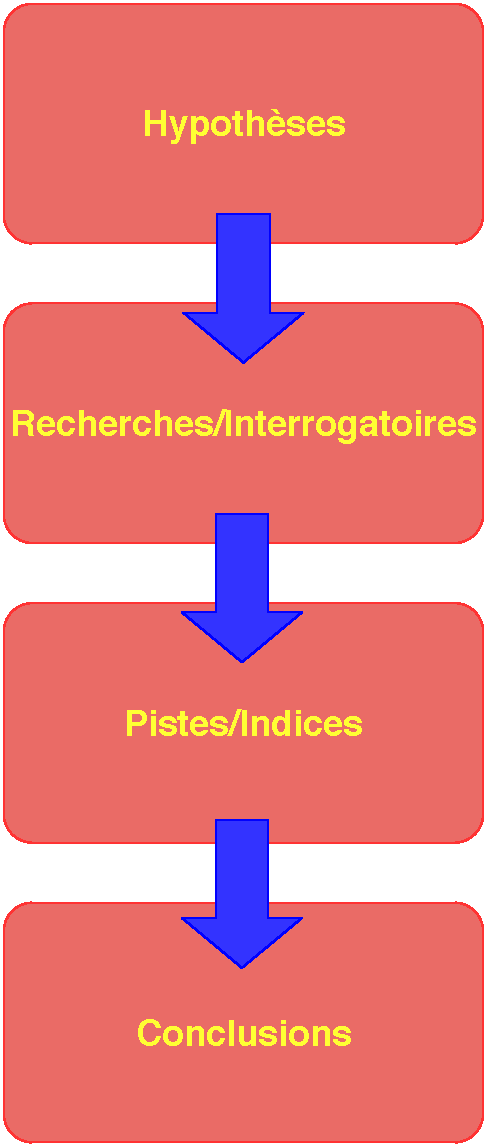
\includegraphics[scale=.4]{images/enth/en4.pdf}}
\end{minipage} \hfill
\begin{minipage}[c]{.46\linewidth}
\only<1>{L'ensemble des connaissances en psychologie, médecine légale, les rapports de police, les techniques d'enquête\dots}
\only<2>{C'est le cœur de la recherche de la vérité, un travail méticuleux basé sur une méthode donnée}
\only<3>{C'est le résultat des recherches, obtenus grâce à la méthode}
\only<4>{On les déduit logiquement des hypothèses \alert{ET} des résultats de la recherche}
\end{minipage}
\end{figure}

\end{frame}


\begin{frame}%[plain]
\frametitle{La recherche scientifique}

\begin{figure}
\begin{minipage}[c]{.46\linewidth}
\only<1>{\hspace{3em}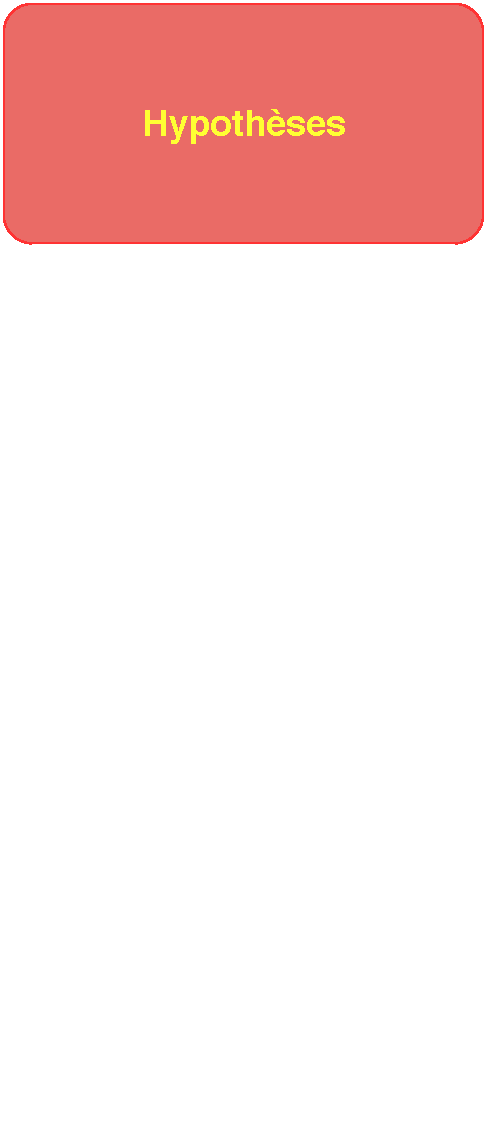
\includegraphics[scale=.4]{images/enth/th1.pdf}}
\only<2>{\hspace{3em}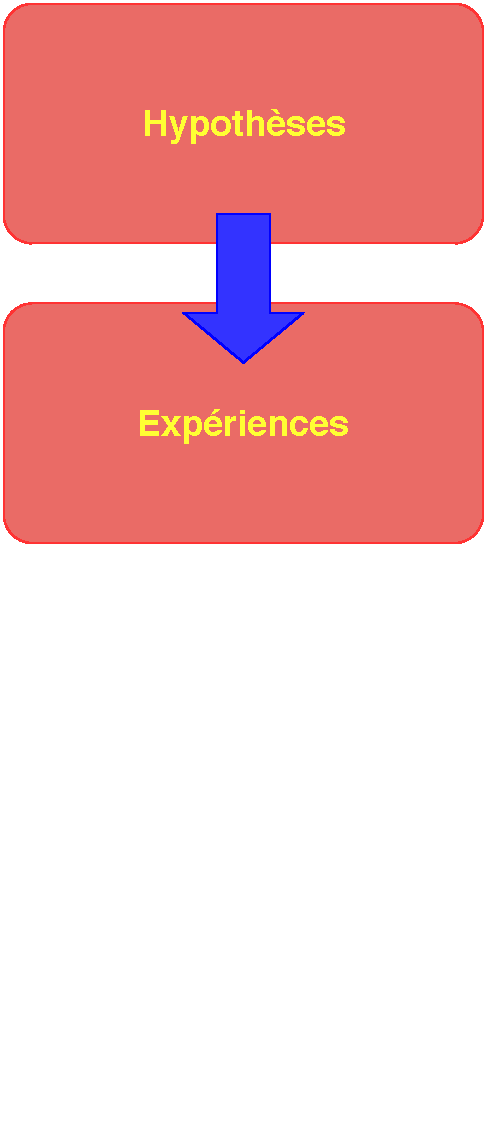
\includegraphics[scale=.4]{images/enth/th2.pdf}}
\only<3>{\hspace{3em}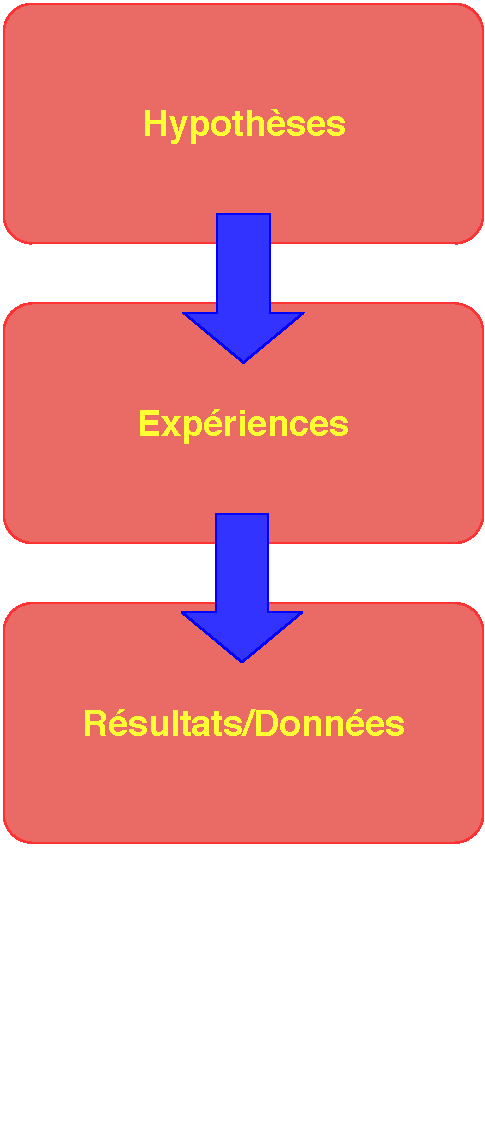
\includegraphics[scale=.4]{images/enth/th3.pdf}}
\only<4>{\hspace{3em}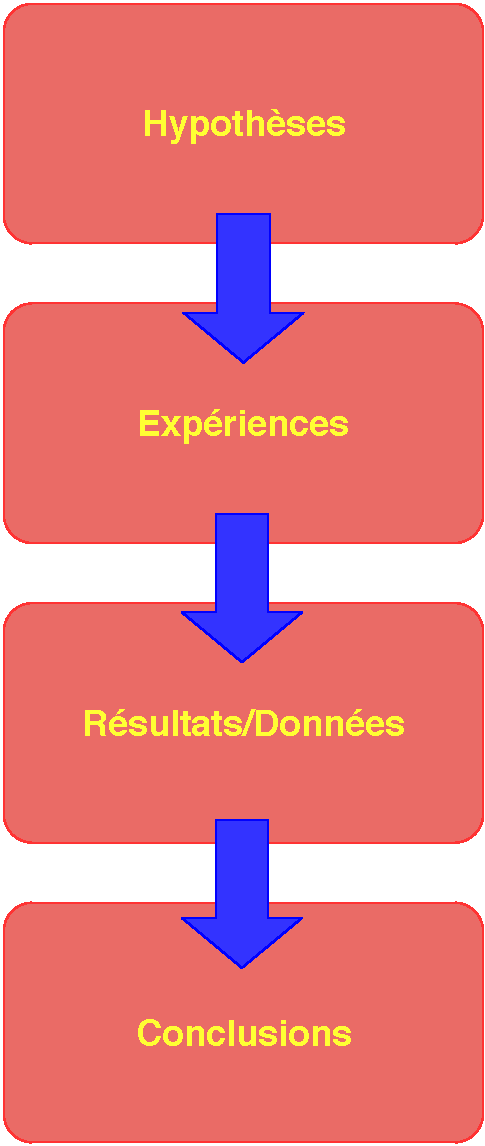
\includegraphics[scale=.4]{images/enth/th4.pdf}}
\end{minipage} \hfill
\begin{minipage}[c]{.46\linewidth}
\only<1>{L'ensemble des connaissances à un moment donné}
\only<2>{Observations et recherche : importance de la méthode de recherche}
\only<3>{Résultats de mesure, de calculs : besoin de leur donner un sens dans le cadre de la théorie}
\only<4>{Conclusions déduites logiquement des hypothèses et des résultats de la recherche}
\end{minipage}
\end{figure}

\end{frame}


\begin{frame}%[plain]


\begin{tikzpicture}
\caneva{12}{9}{white}
\node at (-3.2,-0.1) {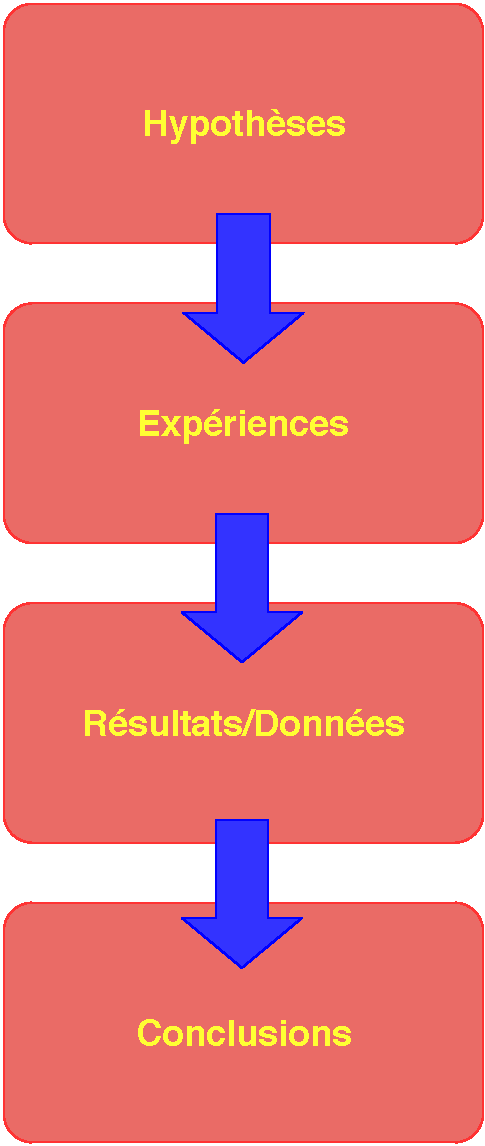
\includegraphics[scale=.4]{images/enth/th4.pdf}};
\node at (3.2,-0.1) {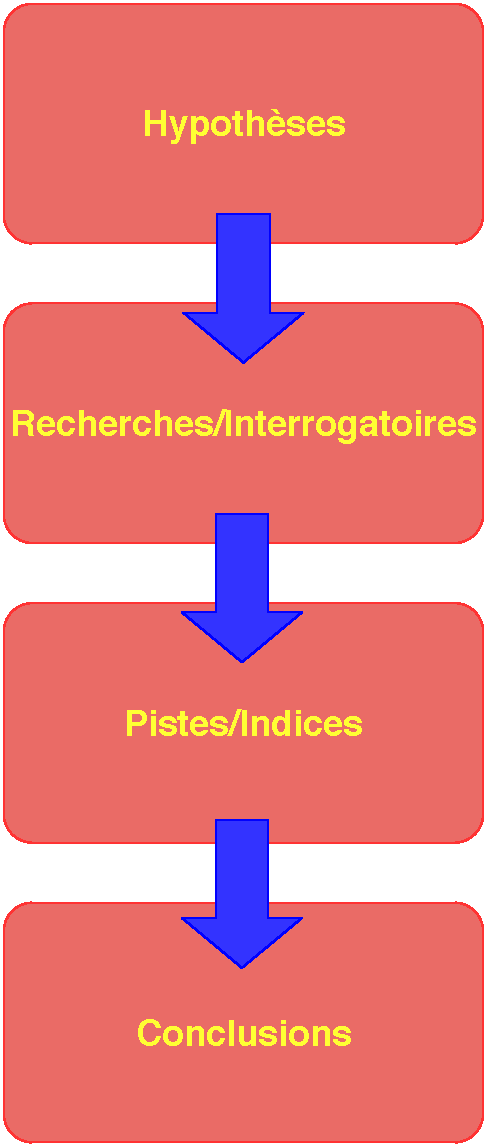
\includegraphics[scale=.4]{images/enth/en4.pdf}};
\node at (-3.2,4) {\textcolor{ForestGreen}{Science}};
\node at (3.2,4) {\textcolor{ForestGreen}{Enquete}};
\only<2->{\draw [very thick, Plum] (-3.2,2.8) ellipse (2 and 1);}
\only<2->{\draw [very thick, Plum] (3.2,2.8) ellipse (2 and 1);}

\only<2->{\draw [very thick, Plum, fill=Plum, opacity=.4] (-3.2,2.8) ellipse (2 and 1);}
\only<2->{\draw [very thick, Plum, fill=Plum, opacity=.4] (3.2,2.8) ellipse (2 and 1);}
\only<2->{\node at (0,2) {\textcolor{Plum}{\Huge Intuition}};}


\only<3->{\draw [very thick, Blue, fill=Blue, opacity=.4] (-3.2,-3.2) ellipse (2 and 1);}
\only<3->{\draw [very thick, Blue, fill=Blue, opacity=.4] (3.2,-3.2) ellipse (2 and 1);}
\only<3->{\draw [very thick, Blue] (-3.2,-3.2) ellipse (2 and 1);}
\only<3->{\draw [very thick, Blue] (3.2,-3.2) ellipse (2 and 1);}
\only<3->{\node at (0,-2.2) {\textcolor{Blue}{\Huge Logique}};}
\end{tikzpicture}


\end{frame}





\begin{frame}%[plain]
\frametitle{Paradoxe de Galilée}

\framesubtitle{\textit{Galileo Galilei} (1564 P.C. - 1642 P.C.)}

\textit{\textbf{Question :}}

Entre deux objets de masses différentes, lequel tombe le plus vite ?

(Le plus lourd ou le plus léger ?)

\onslide<2->{\vspace{1cm}
\textit{\textbf{Réponse :}}

``C'est l'objet le plus lourd qui tombe le plus vite.''

\textit{Aristote} (384 A.C. - 322 A.C.)}

\phantom{\vspace{1cm}}
\phantom{\textit{\textbf{Objection :}}}

\phantom{``Est-ce que quelqu'un aurait un morceau de ficelle ?''}

\phantom{$\approx$\textit{Galileo Galilei} (1564 P.C. - 1642 P.C.)}

\end{frame}


\begin{frame}%[plain]
\begin{center}

\begin{tikzpicture}[background rectangle/.style={fill=cyan}, show background rectangle]
\caneva{5}{8}{cyan}

\only<1>{
\begin{scope}[xshift=-1cm,yshift=3.5cm]
\boule[0.2]{brown}
\draw (0,0) node {\tiny $m_1$};
\end{scope}

\begin{scope}[xshift=1cm,yshift=3.5cm]
\boule[0.4]{brown}
\draw (0,0) node {\scriptsize $m_2$};
\end{scope}
}

\only<2>{
\begin{scope}[xshift=-1cm,yshift=3.cm]
\boule[0.2]{brown}
\draw (0,0) node {\tiny $m_1$};
\end{scope}

\begin{scope}[xshift=1cm,yshift=2.5cm]
\boule[0.4]{brown}
\draw (0,0) node {\scriptsize $m_2$};
\end{scope}
}

\only<3>{
\begin{scope}[xshift=-1cm,yshift=2cm]
\boule[0.2]{brown}
\draw (0,0) node {\tiny $m_1$};
\end{scope}

\begin{scope}[xshift=1cm,yshift=0.5cm]
\boule[0.4]{brown}
\draw (0,0) node {\scriptsize $m_2$};
\end{scope}
}

\only<4>{
\begin{scope}[xshift=-1cm,yshift=1cm]
\boule[0.2]{brown}
\draw (0,0) node {\tiny $m_1$};
\end{scope}

\begin{scope}[xshift=1cm,yshift=-1.5cm]
\boule[0.4]{brown}
\draw (0,0) node {\scriptsize $m_2$};
\end{scope}
}

\end{tikzpicture}

\end{center}
\end{frame}

\begin{frame}%[plain]
\frametitle{Paradoxe de Galilée}
\framesubtitle{\textit{Galileo Galilei} (1564 P.C. - 1642 P.C.)}

\textit{\textbf{Question :}}

Entre deux objets de masses différentes, lequel tombe le plus vite ?

(Le plus lourd ou le plus léger ?)

\vspace{1cm}
\textit{\textbf{Réponse :}}

``C'est l'objet le plus lourd qui tombe le plus vite.''

\textit{Aristote} (384 A.C. - 322 A.C.)

\onslide<2->{\vspace{1cm}
\textit{\textbf{Objection :}}

``Est-ce que quelqu'un aurait un morceau de ficelle ?''

$\approx$\textit{Galileo Galilei} (1564 P.C. - 1642 P.C.)}

\end{frame}

\begin{frame}%[plain]
\begin{center}

\begin{tikzpicture}[background rectangle/.style={fill=cyan}, show background rectangle]

\only<1>{
\caneva{5}{6.8}{cyan}
\begin{scope}[yshift=3.5cm, color=cyan]
\coordinate (A) at (-1,-0.2);
\coordinate (B) at (1,0.4);
\draw (A) .. controls +(0,-0.7) and  +(0,0.7).. (B);
\end{scope}

\begin{scope}[xshift=-1cm,yshift=3.5cm]
\boule[0.2]{brown}
\draw (0,0) node {\tiny $m_1$};
\end{scope}

\begin{scope}[xshift=1cm,yshift=3.5cm]
\boule[0.4]{brown}
\draw (0,0) node {\scriptsize $m_2$};
\end{scope}
}


\only<2>{
\caneva{5}{6.8}{cyan}
\begin{scope}[yshift=3.5cm]
\coordinate (A) at (-1,-0.2);
\coordinate (B) at (1,0.4);
\draw (A) .. controls +(0,-0.7) and  +(0,0.7).. (B);
\end{scope}

\begin{scope}[xshift=-1cm,yshift=3.5cm]
\boule[0.2]{brown}
\draw (0,0) node {\tiny $m_1$};
\end{scope}

\begin{scope}[xshift=1cm,yshift=3.5cm]
\boule[0.4]{brown}
\draw (0,0) node {\scriptsize $m_2$};
\end{scope}
}

\only<3>{
\caneva{5}{7.4}{cyan}
\begin{scope}[yshift=3.7cm,color=cyan]
\coordinate (A) at (-1,-0.2);
\coordinate (B) at (1,-0.1);
\draw (A) .. controls +(0,-0.7) and  +(0,0.7).. (B);
\end{scope}

\begin{scope}[yshift=3.cm]
\coordinate (A) at (-1,-0.2);
\coordinate (B) at (1,-0.1);
\draw (A) .. controls +(0,-0.7) and  +(0,0.7).. (B);
\end{scope}

\begin{scope}[xshift=-1cm,yshift=3.cm]
\boule[0.2]{brown}
\draw (0,0) node {\tiny $m_1$};
\end{scope}

\begin{scope}[xshift=1cm,yshift=2.5cm]
\boule[0.4]{brown}
\draw (0,0) node {\scriptsize $m_2$};
\end{scope}
}

\only<4>{
\caneva{5}{8}{cyan}
\begin{scope}[yshift=2cm]
\coordinate (A) at (-1,-0.2);
\coordinate (B) at (1,-1.1);
\draw (A) .. controls +(0,-0.7) and  +(0,0.7).. (B);
\end{scope}

\begin{scope}[xshift=-1cm,yshift=2cm]
\boule[0.2]{brown}
\draw (0,0) node {\tiny $m_1$};
\end{scope}

\begin{scope}[xshift=1cm,yshift=0.5cm]
\boule[0.4]{brown}
\draw (0,0) node {\scriptsize $m_2$};
\end{scope}
}

\only<5->{
\caneva{5}{8}{cyan}
\begin{scope}[yshift=1cm]
\coordinate (A) at (-1,-0.2);
\coordinate (B) at (1,-2.1);
\draw (A) .. controls +(0,-0.2) and  +(0,0.2).. (B);
\end{scope}

\begin{scope}[xshift=-1cm,yshift=1cm]
\boule[0.2]{brown}
\draw (0,0) node {\tiny $m_1$};
\end{scope}

\begin{scope}[xshift=1cm,yshift=-1.5cm]
\boule[0.4]{brown}
\draw (0,0) node {\scriptsize $m_2$};
\end{scope}
}

\only<6>{\draw (0.,0.) node[above] {\color{red} $?$};}

\end{tikzpicture}

\end{center}
\end{frame}

\begin{frame}%[plain]
\frametitle{Paradoxe de Galilée}
\framesubtitle{\textit{Galileo Galilei} (1564 P.C. - 1642 P.C.)}

\vspace{-8mm}
\begin{center}
``C'est l'objet le plus lourd qui tombe le plus vite.''
\end{center}

L'objet $2$ (de masse $m_2$) est plus lourd que l'objet $1$ (de masse $m_1$).

$\Rightarrow$ L'objet $2$ tombe plus vite que l'objet $1$.

\onslide<2->{$\Rightarrow$ La ficelle va se tendre et, comme l'objet de masse $m_1$ tombe moins vite, il va freiner l'objet de masse $m_2$.}

\onslide<3->{$\Rightarrow$ Le système (objet $1$ + objet $2$) tombe \emph{moins vite} que l'objet $2$ seul.}

\onslide<4->{\vspace{2mm}
\textbf{\MakeUppercase{Oui mais}}
\vspace{2mm}}

\onslide<5->{Le système (objet $1$ + objet $2$) se déplace comme un seul objet de masse $m_1 + m_2$.

$\Rightarrow$ Le système est plus lourd que l'objet $2$ seul.

$\Rightarrow$ Le système (objet $1$ + objet $2$) tombe \emph{plus vite} que l'objet $2$ seul.}

\end{frame}

\begin{frame}%[plain]
\frametitle{Paradoxe de Galilée}
\framesubtitle{\textit{Galileo Galilei} (1564 P.C. - 1642 P.C.)}

Autrement dit \dots

Si les objets plus lourds tombent \emph{plus vite} que les objets plus légers, \textbf{alors} les objets plus lourds tombent \emph{moins vite} que les objets plus légers.

\onslide<2->{\vspace{2mm}
Qu'est-ce que \dots~quoi ?}

\onslide<3->{\begin{center}
  \Large Impossibilité logique !
%
  %(Résultat absurde)
\end{center}}

\end{frame}

\begin{frame}%[plain]
\frametitle{Paradoxe de Galilée : Solution}
\framesubtitle{\textit{Galileo Galilei} (1564 P.C. - 1642 P.C.)}

Comment résoudre ce ``paradoxe'' ?

\begin{itemize}
\onslide<2->{\item[$\hookrightarrow$] L'hypothèse d'Aristote mène à un résultat contradictoire (absurde)

\item[$\Rightarrow$] On \textbf{ne} peut \textbf{pas} considérer que de deux objets, le plus lourd est celui qui tombe le plus vite}

\onslide<3->{\item[$\hookrightarrow$] L'hypothèse inverse mène à la même contradiction

\item[$\Rightarrow$] On \textbf{ne} peut \textbf{pas} non plus considérer que de deux objets, le plus léger est celui qui tombe le plus vite}

\onslide<4->{\item[$\hookrightarrow$] Seule solution : Tous les objets tombent à la même vitesse, indépendement de leur masse.}

\end{itemize}

\onslide<5->{En fait, le ``paradoxe de Galilée'' est une \textbf{preuve par l'absurde} du fait que tous les objets tombent à la même vitesse, indépendement de leur masse.}

\end{frame}


\begin{frame}%[plain]
\frametitle{Paradoxe de Galilée : Pourquoi cette fausse conception ?}
\framesubtitle{\textit{Galileo Galilei} (1564 P.C. - 1642 P.C.)}

Même si l'on est convaincu par le raisonnement de Galilée, on avait naturellement tendance à penser que les objets plus lourds tombent plus vite.

D'où nous vient cette intuition éronnée ?

\onslide<2->{%
\begin{itemize}
\item[$\boldsymbol{\rightarrow}$] Dans la vie de tous les jours, on a quand même de bonnes raisons de penser que les objets plus lourds tombent plus vite. \\ (ex : lâcher d'un marteu et d'une plume)
\item[$\boldsymbol{\rightarrow}$] La vie de tous les jours = sur Terre = \textbf{dans l'air !}
\begin{itemize}
\item Présence de \textbf{forces de frottement} dues à l'air.
\item Ces forces de forttement sont \textbf{proportionnelles à la surface} de l'objet en mouvement.
\end{itemize}
\item[\color{white}$\boldsymbol{\rightarrow}$]\phantom{Si l'on fait lexpérience \textbf{en l'absence d'air} (ex : sur la Lune), on observe bien que \textbf{des objets lâchés en même temps tombent à la même vitesse} à tout instant.}
\end{itemize}}

\end{frame}

\begin{frame}%[plain]
\frametitle{Paradoxe de Galilée : Pourquoi cette fausse conception ?}
\framesubtitle{Vue d'artiste}
\vspace{-1cm}
\begin{center}
\begin{tikzpicture}[background rectangle/.style={fill=cyan}, show background rectangle]
\caneva{8}{7.5}{cyan}
\draw (0,2.5) node{\color{umons-red}Round 1};
%Ajout d'un élément invisible pour fixer la taille du cadre
\draw[color=cyan,fill=cyan,yshift=3.3cm,scale=0.5] (1,0) arc (0:180: 1);
%C'est sale... Mis ça marche

\only<1>{
\begin{scope}[yshift=2.5cm]
\begin{scope}[xshift=-2cm,yshift=0.8cm,scale=0.5]
\parachute
\end{scope}
\draw (-2,0) node{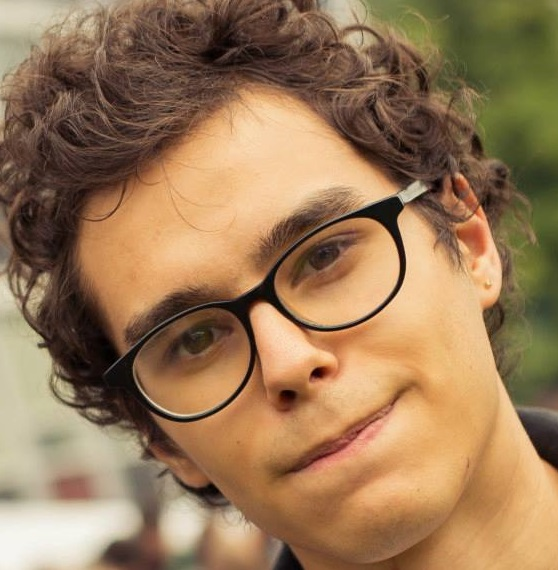
\includegraphics[scale=0.05]{images/antoine.jpg}};
\end{scope}
\begin{scope}[yshift=2.5cm]
\draw (2,0) node{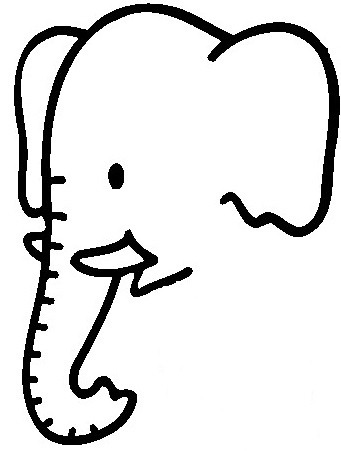
\includegraphics[scale=0.08]{images/elephant.jpg}};
\end{scope}
}

\only<2>{
\begin{scope}[yshift=2.3cm]
\begin{scope}[xshift=-2cm,yshift=0.8cm,scale=0.5]
\parachute
\end{scope}
\draw (-2,0) node{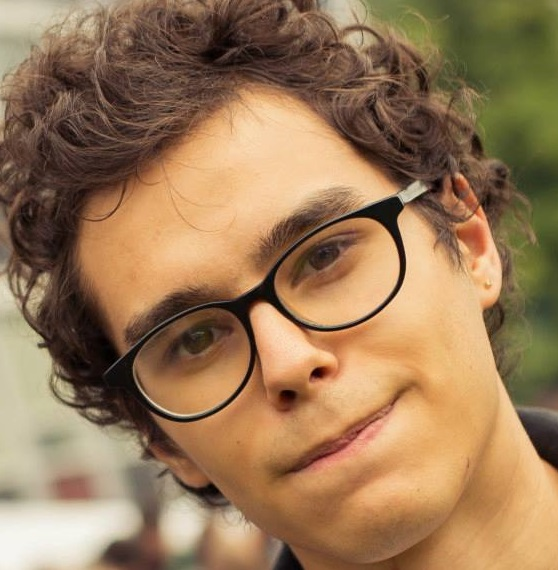
\includegraphics[scale=0.05]{images/antoine.jpg}};
\end{scope}
\begin{scope}[yshift=2.cm]
\draw (2,0) node{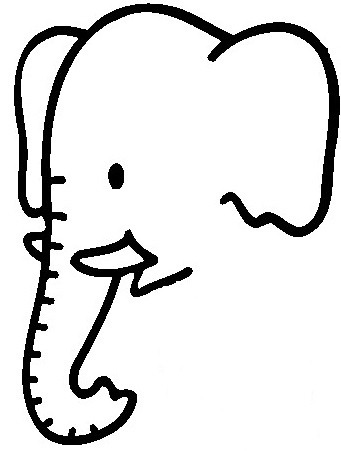
\includegraphics[scale=0.08]{images/elephant.jpg}};
\end{scope}
}

\only<3>{
\begin{scope}[yshift=2.1cm]
\begin{scope}[xshift=-2cm,yshift=0.8cm,scale=0.5]
\parachute
\end{scope}
\draw (-2,0) node{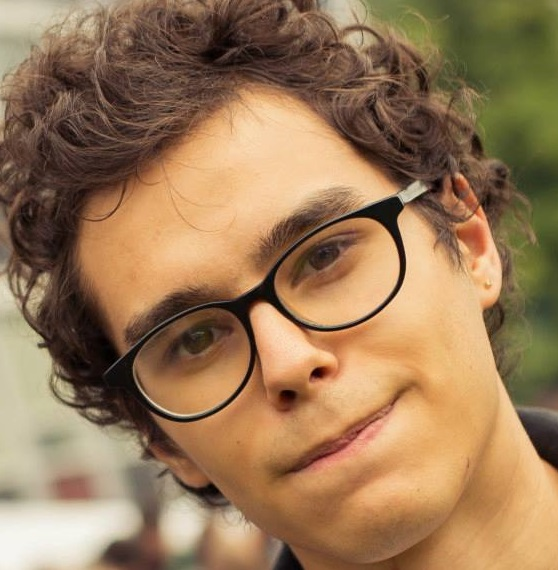
\includegraphics[scale=0.05]{images/antoine.jpg}};
\end{scope}
\begin{scope}[yshift=1.5cm]
\draw (2,0) node{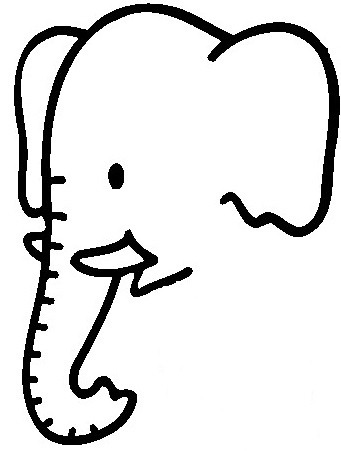
\includegraphics[scale=0.08]{images/elephant.jpg}};
\end{scope}
}

\only<4>{
\begin{scope}[yshift=1.8cm]
\begin{scope}[xshift=-2cm,yshift=0.8cm,scale=0.5]
\parachute
\end{scope}
\draw (-2,0) node{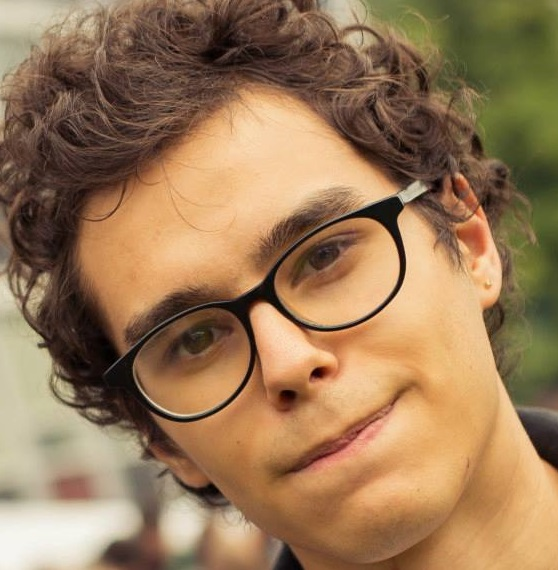
\includegraphics[scale=0.05]{images/antoine.jpg}};
\end{scope}
\begin{scope}[yshift=0.4cm]
\draw (2,0) node{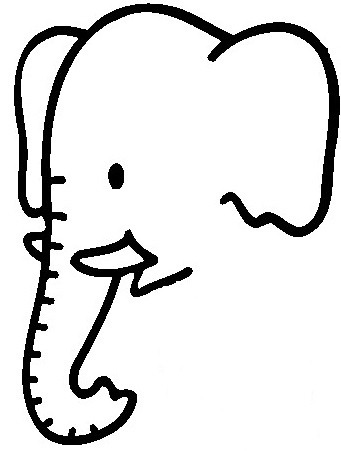
\includegraphics[scale=0.08]{images/elephant.jpg}};
\end{scope}
}

\only<5>{
\begin{scope}[yshift=1.5cm]
\begin{scope}[xshift=-2cm,yshift=0.8cm,scale=0.5]
\parachute
\end{scope}
\draw (-2,0) node{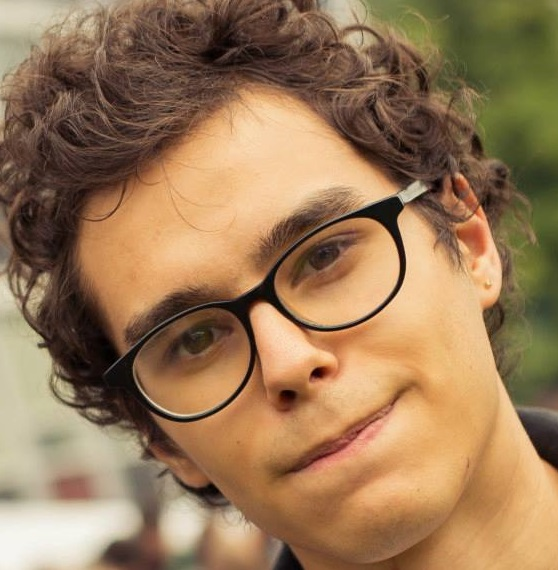
\includegraphics[scale=0.05]{images/antoine.jpg}};
\end{scope}
\begin{scope}[yshift=-0.5cm]
\draw (2,0) node{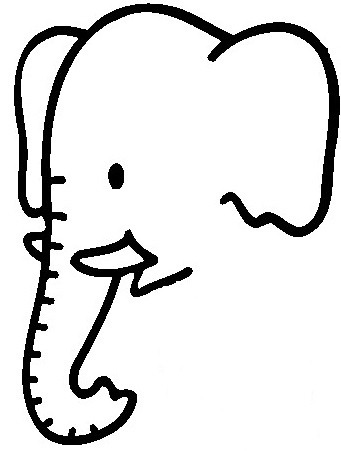
\includegraphics[scale=0.08]{images/elephant.jpg}};
\end{scope}
}


\only<6>{
\begin{scope}[yshift=1cm]
\begin{scope}[xshift=-2cm,yshift=0.8cm,scale=0.5]
\parachute
\end{scope}
\draw (-2,0) node{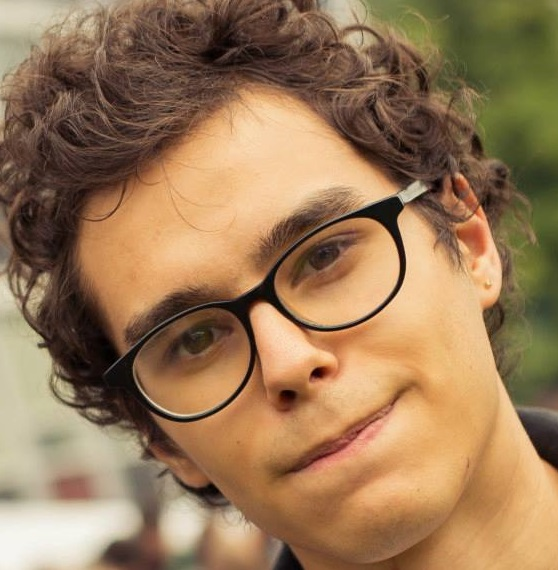
\includegraphics[scale=0.05]{images/antoine.jpg}};
\end{scope}
\begin{scope}[yshift=-1.5cm]
\draw (2,0) node{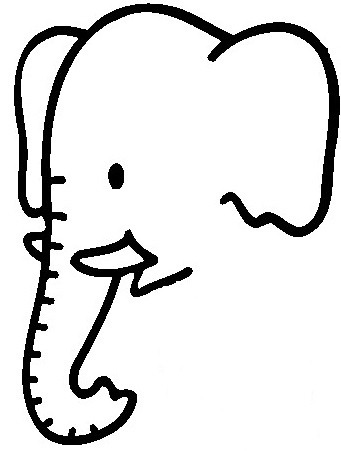
\includegraphics[scale=0.08]{images/elephant.jpg}};
\end{scope}
}


\only<6>{\draw (0,-2.5) node{\color{umons-red}$\Rightarrow$ L'élephant s'écrase sur le sol};}
\draw (0,-3.5) node{\phantom{\color{umons-red}$\leftrightarrow$ Force de frottement de l'air sur le parachute}};
\end{tikzpicture}
\end{center}
\end{frame}


\begin{frame}%[plain]
\frametitle{Paradoxe de Galilée : Pourquoi cette fausse conception ?}
\framesubtitle{Vue d'artiste}
\vspace{-1cm}
\begin{center}
\begin{tikzpicture}[background rectangle/.style={fill=cyan}, show background rectangle]
\caneva{8}{7.5}{cyan}
\draw (0,2.5) node{\color{umons-red}Round 2};
%Ajout d'un élément invisible pour fixer la taille du cadre
\draw[color=cyan,fill=cyan,yshift=3.3cm,scale=0.5] (1,0) arc (0:180: 1);
%C'est sale... Mis ça marche


\only<1>{
\begin{scope}[yshift=2.5cm]
\begin{scope}[xshift=-2cm,yshift=0.8cm,scale=0.5]
\parachute
\end{scope}
\draw (-2,0) node{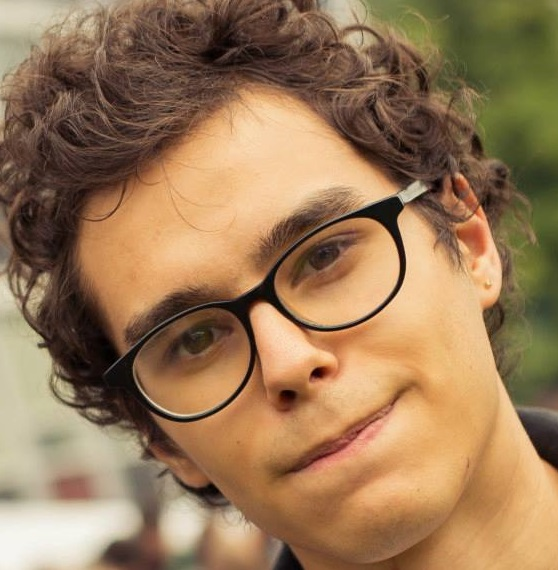
\includegraphics[scale=0.05]{images/antoine.jpg}};
\end{scope}
\begin{scope}[yshift=2.5cm]
\draw (2,0) node{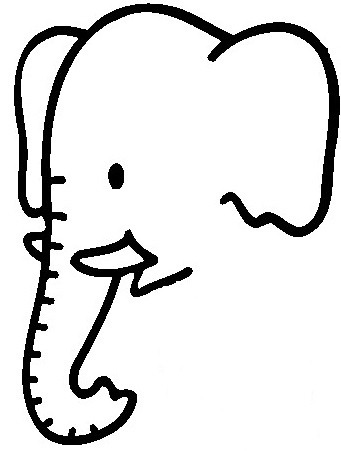
\includegraphics[scale=0.08]{images/elephant.jpg}};
\end{scope}
}

\only<2>{
\begin{scope}[yshift=2.5cm]
\draw (-2,0) node{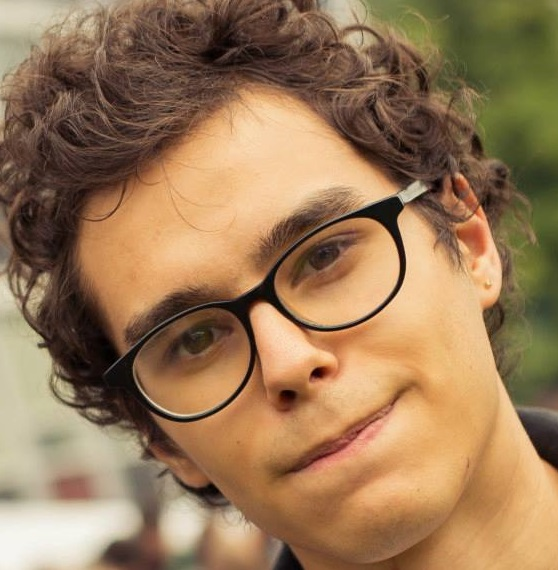
\includegraphics[scale=0.05]{images/antoine.jpg}};
\end{scope}
\begin{scope}[yshift=2.5cm]
\begin{scope}[xshift=2cm,yshift=0.8cm,scale=0.5]
\parachute
\end{scope}
\draw (2,0) node{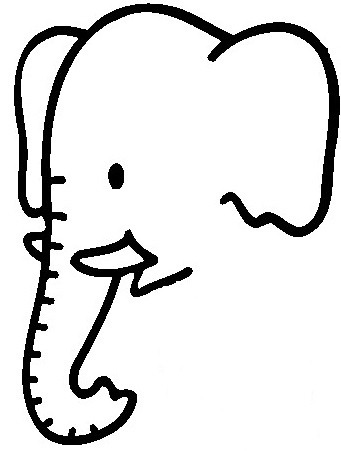
\includegraphics[scale=0.08]{images/elephant.jpg}};
\end{scope}
}

\only<3>{
\begin{scope}[yshift=2.5cm]
\draw (-2,0) node{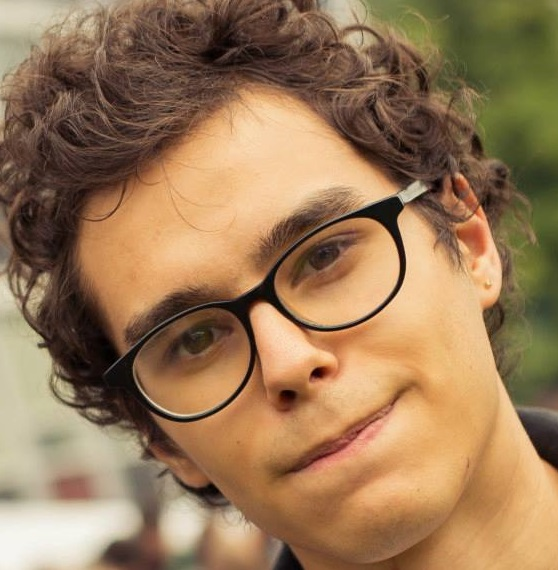
\includegraphics[scale=0.05]{images/antoine.jpg}};
\draw (-0.97,0.4) node{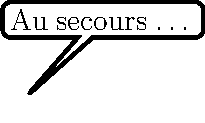
\includegraphics[scale=0.5]{images/help.pdf}};
\end{scope}
\begin{scope}[yshift=2.5cm]
\begin{scope}[xshift=2cm,yshift=0.8cm,scale=0.5]
\parachute
\end{scope}
\draw (2,0) node{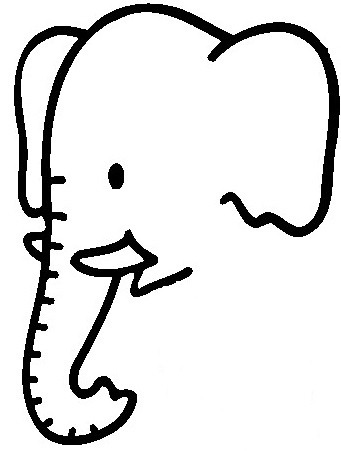
\includegraphics[scale=0.08]{images/elephant.jpg}};
\end{scope}
}

\only<4>{
\begin{scope}[yshift=2.06cm]
\draw (-2,0) node{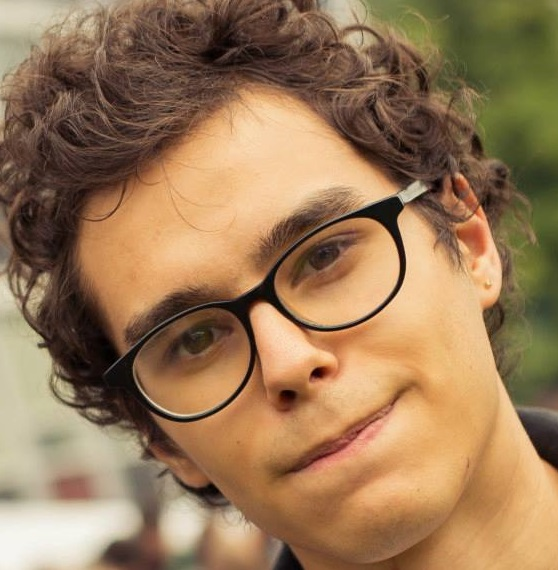
\includegraphics[scale=0.05]{images/antoine.jpg}};
\draw (-0.97,0.4) node{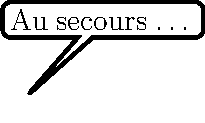
\includegraphics[scale=0.5]{images/help.pdf}};
\end{scope}
\begin{scope}[yshift=2.3cm]
\begin{scope}[xshift=2cm,yshift=0.8cm,scale=0.5]
\parachute
\end{scope}
\draw (2,0) node{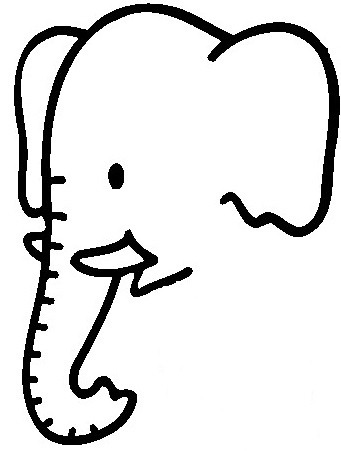
\includegraphics[scale=0.08]{images/elephant.jpg}};
\end{scope}
}

\only<5>{
\begin{scope}[yshift=1.4cm]
\draw (-2,0) node{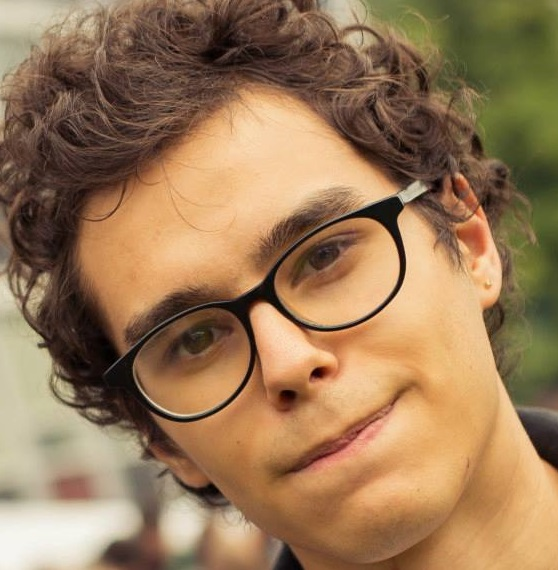
\includegraphics[scale=0.05]{images/antoine.jpg}};
\draw (-0.97,0.4) node{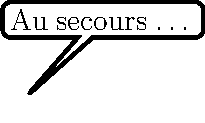
\includegraphics[scale=0.5]{images/help.pdf}};
\end{scope}
\begin{scope}[yshift=2.1cm]
\begin{scope}[xshift=2cm,yshift=0.8cm,scale=0.5]
\parachute
\end{scope}
\draw (2,0) node{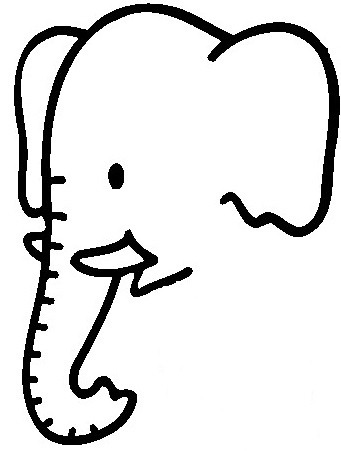
\includegraphics[scale=0.08]{images/elephant.jpg}};
\end{scope}
}

\only<6>{
\begin{scope}[yshift=0.4cm]
\draw (-2,0) node{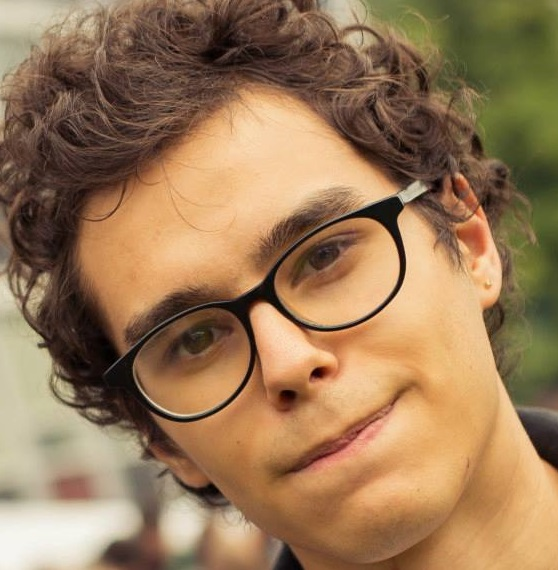
\includegraphics[scale=0.05]{images/antoine.jpg}};
\draw (-0.97,0.4) node{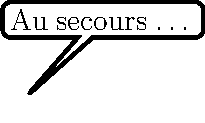
\includegraphics[scale=0.5]{images/help.pdf}};
\end{scope}
\begin{scope}[yshift=1.8cm]
\begin{scope}[xshift=2cm,yshift=0.8cm,scale=0.5]
\parachute
\end{scope}
\draw (2,0) node{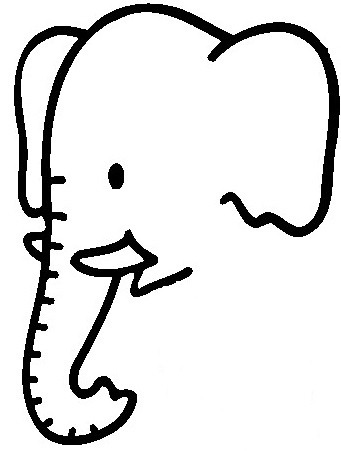
\includegraphics[scale=0.08]{images/elephant.jpg}};
\end{scope}
}

\only<7>{
\begin{scope}[yshift=-0.5cm]
\draw (-2,0) node{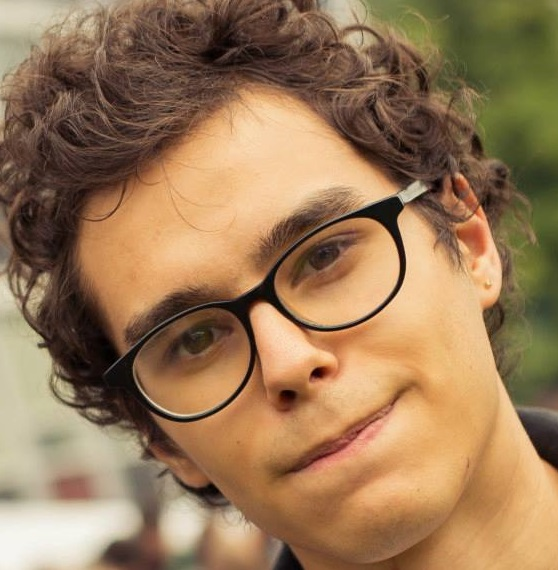
\includegraphics[scale=0.05]{images/antoine.jpg}};
\draw (-0.97,0.4) node{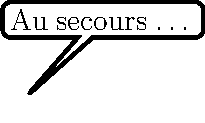
\includegraphics[scale=0.5]{images/help.pdf}};
\end{scope}
\begin{scope}[yshift=1.5cm]
\begin{scope}[xshift=2cm,yshift=0.8cm,scale=0.5]
\parachute
\end{scope}
\draw (2,0) node{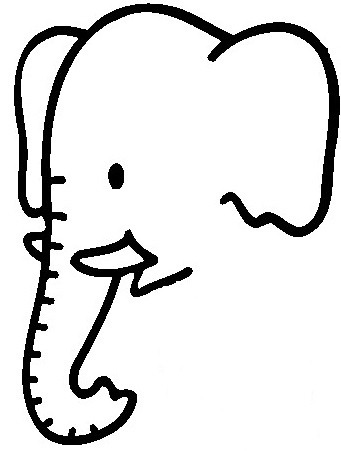
\includegraphics[scale=0.08]{images/elephant.jpg}};
\end{scope}
}

\only<8->{
\begin{scope}[yshift=-1.5cm]
\draw (-2,0) node{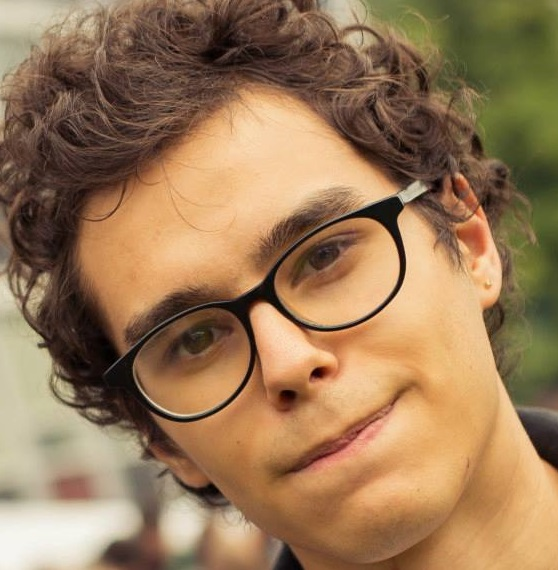
\includegraphics[scale=0.05]{images/antoine.jpg}};
\draw (-0.97,0.4) node{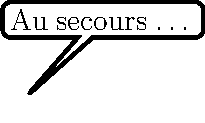
\includegraphics[scale=0.5]{images/help.pdf}};
\end{scope}
\begin{scope}[yshift=1.cm]
\begin{scope}[xshift=2cm,yshift=0.8cm,scale=0.5]
\parachute
\end{scope}
\draw (2,0) node{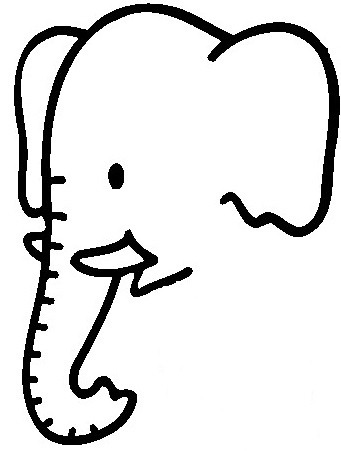
\includegraphics[scale=0.08]{images/elephant.jpg}};
\end{scope}
}

%\only<8->{\draw (-1.08,-1) node{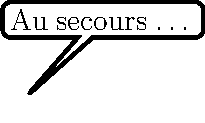
\includegraphics[scale=0.5]{images/help.pdf}};}
\only<8->{\draw (0,-2.5) node{\color{umons-red}$\Rightarrow$ L'élephant arrive en bas en un seul morceau};}
\only<9>{\draw (0,-3) node{\color{umons-red}$\rightarrow$ Seule différence : qui porte le parachute};}
\onslide<9>{\draw (0,-3.5) node{\color{umons-red}$\leftrightarrow$ Force de frottement de l'air sur le parachute};}
\end{tikzpicture}
\end{center}
\end{frame}

\begin{frame}%[plain]
\frametitle{Paradoxe de Galilée : Pourquoi cette fausse conception ?}
\framesubtitle{\textit{Galileo Galilei} (1564 P.C. - 1642 P.C.)}

Même si l'on est convaincu par le raisonnement de Galilée, on avait naturellement tendance à penser que les objets plus lourds tombent plus vite.

D'où nous vient cette intuition éronnée ?

\begin{itemize}
\item[$\boldsymbol{\rightarrow}$] Dans la vie de tous les jours, on a quand même de bonnes raisons de penser que les objets plus lourds tombent plus vite. \\ (ex : lâcher d'un marteu et d'une plume)
\item[$\boldsymbol{\rightarrow}$] La vie de tous les jours = sur Terre = \textbf{dans l'air !}
\begin{itemize}
\item Présence de \textbf{forces de frottement} dues à l'air.
\item Ces forces de forttement sont \textbf{proportionnelles à la surface} de l'objet en mouvement.
\end{itemize}
\onslide<2->{\item[$\boldsymbol{\rightarrow}$]Si l'on fait lexpérience \textbf{en l'absence d'air} (ex : sur la Lune), on observe bien que \textbf{des objets lâchés en même temps tombent à la même vitesse} à tout instant.}
\end{itemize}

\end{frame}




\begin{frame}%[plain]
{Paradoxe de Zénon}
\pause Ou la fable du lièvre et de la tortue par Zénon d'\'{E}lée en 450 ACN
\pause  \vspace{0.5cm}
\\ \color{umons-red} \textbf{\'{E}noncé du} \textit{paradoxe}
\pause
\begin{tabular}{cccc|}
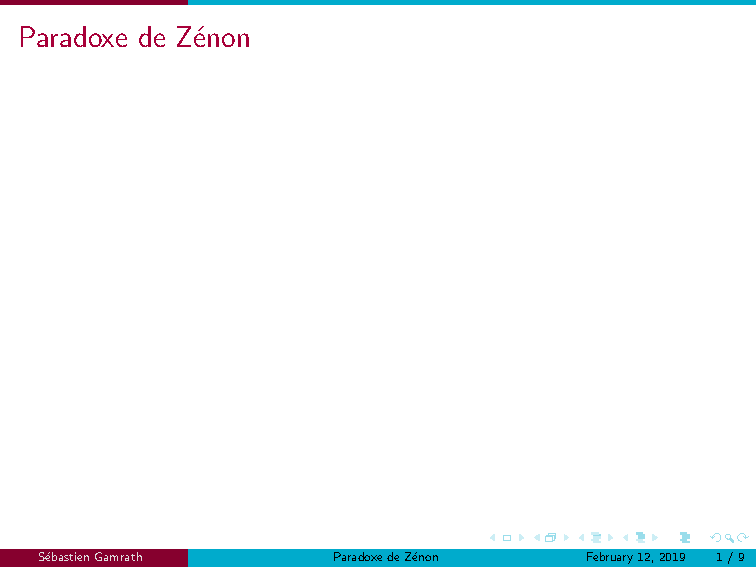
\includegraphics[scale=0.2]{images/Zenon.jpg}\pause    & \includegraphics[scale=0.49]{images/Achilles.jpg} \pause & \includegraphics[scale=0.08]{images/piste.jpg} \pause & \includegraphics[scale=0.07]{images/tortue.jpg}  \\ 
\end{tabular} 
\end{frame}





\begin{frame}%[plain]
{Paradoxe de Zénon}
Ou la fable du lièvre et de la tortue par Zénon d'\'{E}lée en 450 ACN
\vspace{0.5cm}
\\ \color{umons-red} \textbf{\'{E}noncé du} \textit{paradoxe}
\\ \color{black}Le paradoxe d'Achille et de la tortue tel que formulé par Zénon dit qu'un jour, Achille, le héros grec, disputa une course avec une tortue. Achille étant un athlète de bon niveau et étant bon joueur, il laisse un avance à la tortue. Zénon affirme qu'il ne pourra jamais rattraper le lent reptile. En effet, bien qu'Achille court beaucoup plus vite, le temps qu'il parcourt la distance qu'il a laissé à la tortue, cette dernière a parcouru une certaine distance non nulle donc elle a encore de l'avance. Le temps qu'Achille rattrape ce retard, la tortue a encore avancé et le processus est itéré. Achille ne rattrape donc jamais la tortue.
\end{frame}



\begin{frame}%[plain]
{Paradoxe de Zénon}
Peut-être sera-ce plus clair sur cette figure : 
\begin{center}
\includegraphics[scale=0.2]{images/ZAPT1.png}
\end{center}
\end{frame}





\begin{frame}%[plain]
{Paradoxe de Zénon}
Une autre manière de voir le paradoxe
\begin{center}
\begin{overpic}[scale=0.5]{images/glass1.png}
\put(80,20){\huge$\frac{1}{2}$}
\end{overpic}
%\includegraphics[scale=0.5]{images/glass1.png}
\end{center}
\end{frame}





\begin{frame}%[plain]
{Paradoxe de Zénon}
Une autre manière de voir le paradoxe
\begin{center}
\begin{overpic}[scale=0.5]{images/glass2.png}
\put(80,20){\huge$\frac{1}{2}$}
\put(80,40){\Large$+$}
\put(80,55){\huge$\frac{1}{4}$}
\end{overpic}
%\includegraphics[scale=0.5]{images/glass2.png}
\end{center}
\end{frame}



\begin{frame}%[plain]
{Paradoxe de Zénon}
Une autre manière de voir le paradoxe
\begin{center}
\begin{overpic}[scale=0.5]{images/glass3.png}
\put(80,20){\huge$\frac{1}{2}$}
\put(80,40){\Large$+$}
\put(80,55){\huge$\frac{1}{4}$}
\put(80,67){\large$+$}
\put(80,75){\Large$\frac{1}{8}$}
\end{overpic}
%\includegraphics[scale=0.5]{images/glass3.png}
\end{center}
\end{frame}






\begin{frame}%[plain]
{Paradoxe de Zénon}
Une autre manière de voir le paradoxe
\begin{center}
\begin{overpic}[scale=0.5]{images/glass4.png}
\put(80,20){\huge$\frac{1}{2}$}
\put(80,40){\Large$+$}
\put(80,55){\huge$\frac{1}{4}$}
\put(80,67){\large$+$}
\put(80,75){\Large$\frac{1}{8}$}
\put(80,85){\large$+$}
\put(80,95){\Large$\vdots$}
\end{overpic}
%\includegraphics[scale=0.5]{images/glass4.png}
\end{center}
\end{frame}



\begin{frame}%[plain]
{Paradoxe de Zénon}
Une autre manière de voir le paradoxe
\begin{center}
\begin{overpic}[scale=0.5]{images/glass5.png}
\put(80,20){\huge$\frac{1}{2}$}
\put(80,40){\Large$+$}
\put(80,55){\huge$\frac{1}{4}$}
\put(80,67){\large$+$}
\put(80,75){\Large$\frac{1}{8}$}
\put(80,85){\large$+$}
\put(80,95){\Large$\vdots$}
\end{overpic}
%\includegraphics[scale=0.5]{images/glass5.png}
\end{center}
\end{frame}




\begin{frame}%[plain]
{Paradoxe de Zénon}
Retour à la course entre Achille et la tortue 
\pause
\begin{center}
\includegraphics[scale=0.35]{images/ZAPT2.png}
\end{center}
\end{frame}



\begin{frame}%[plain]
{Paradoxe de Zénon}
Retour à la course entre Achille et la tortue
\begin{center}
\includegraphics[scale=0.35]{images/ZAPT3.png}
\end{center}
\end{frame}




\begin{frame}%[plain]
{Paradoxe de Zénon}
{Séries convergentes :}
% \\
Si Achille se déplace à 10 m/s et la tortue à 5 m/s et qu'initialement la distance entre les deux vaut 100m, alors on a à résoudre : 
\only<1>{\[T  = 10 + \frac{10}{2} +  \frac{10}{4} + \frac{10}{8} + \cdots \]}
\only<2>{\[T = 10 \left(1 + \frac{1}{2} +  \frac{1}{4} + \frac{1}{8} + \cdots\right)\]}
\only<3->{\[T = 10 \left(\left(\frac{1}{2}\right)^{0} + \left(\frac{1}{2}\right)^{1} +  \left(\frac{1}{2}\right)^2 + \left(\frac{1}{2}\right)^3 + \cdots\right)\]} %\pause
\onslide<4->{Autrement dit :
\[ T = 10 \sum_{n=0}^{\infty} \left(\frac{1}{2}\right)^{n}\]
C'est la somme d'une série géométrique : \[\sum_{k=0}^{\infty} x^k = \frac{1}{1-x}\onslide<5->{, \text{ si} \left\vert x \right\vert < 1 \]}} %\pause 
\onslide<6->{Donc dans notre cas : \[ T = 10 \cdot \frac{1}{1- 1/2} = 10\cdot 2 = 20 \]}
\end{frame}

\begin{frame}%[plain]
\frametitle{Une maladie bien inquiétante\dots}

Imaginons la situation suivante :

\begin{itemize}
\item Une maladie terrible touche en moyenne 1/10000 personne
\item Il existe un test fiable à $99\%$ \pause
\begin{itemize}
\item Si vous êtes malade : dans $99\%$ des cas le test est \positif
\item Si vous n'êtes pas malade : dans $99\%$ des cas le test est \negatif
\end{itemize}
\item Par précaution, vous passez le test : il est \positif \pause
\item Qu'est-ce que vous faites ? \pause
\end{itemize}

$\Rightarrow$ On voudrait connaître la probabilité d'être vraiment malade après un test \positif

\end{frame}

\begin{frame}%[plain]
\frametitle{Du calme et prenons du recul : formule de Bayes}

\pause

On pose :

\begin{itemize}
\item A : vous êtes malade
\item B : test \positif
\end{itemize}

\pause

On peut utiliser la \alert{Formule de Bayes} :

\[
P(A|B) = \frac{P(B|A)P(A)}{P(B)}
\]

\pause
$P(A)$ : probabilité d'être malade

$P(B)$ : probabilité d'avoir un test \positif\pause

$P(A|B)$ (proba de $A$ sachant $B$) : probabilité d'être malade en ayant un test \positif\pause

$P(B|A)$ : probabilité d'avoir un test \positif si on est malade %\pause

\end{frame}

\begin{frame}%[plain]
\frametitle{Raisonnons étape par étape}

On connaît quoi, dans toute cette histoire ?

\begin{itemize}
\item $P(A) = \frac{1}{10000}$ \pause
\item $P(B|A) = 0.99$ \pause
\item $P(A|B) = ??$ \pause
\item $P(B) = ??$ \pause

\begin{align*}P(B) &= P(A)P(B|A) + P(\bar{A})P(B|\bar{A})\\
&=\frac{1}{10000}0.99 + \frac{9999}{10000}0.01\\
&= 0.010098 \approx 1\%\end{align*}

\end{itemize}

Notons que $P(A)$ et $P(B)$ sont des probabilités \textit{a priori}

\end{frame}





\begin{frame}%[plain]
\frametitle{Résultat des courses}

On remet tout ça dans la formule de Bayes et on obtient :

\begin{align*}
P(A|B) &= \frac{P(B|A)P(A)}{P(B)}\\
&= \frac{0.99 \times 0.0001}{0.010098} = 0.0099 \approx 1\%
\end{align*}


\pause
La probabilité d'être malade en ayant un test \positif est d'environ $1\%$

\pause

\begin{itemize}
\item Dans la réalité : impossible d'avoir un test fiable à $100\%$ \pause
\item On peut utiliser les probabilités pour analyser une situation réelle et décider de la marche à suivre \pause
\item On a tendance à réagir de manière non rationnelle\pause
\item Un peu de réflexion remet de l'ordre là-dedans%\pause
\end{itemize}


\end{frame}


\begin{frame}%[plain]
\frametitle{Pourquoi cette erreur ?}



\only<5>{\[
P(A|B) = \frac{P(B|A)\cancel{\textcolor{Red}{P(A)}}}{\cancel{\textcolor{Red}{P(B)}}}
\]
}

\only<1-4>{\[
P(A|B) = \frac{P(B|A)P(A)}{P(B)}
\]
}


\vspace{2cm}

\begin{itemize}
\item<2-> On a tendance à se focaliser sur la dernière information
\item<3-> On oublie le contexte
\item<4-> On néglige les probabilités \textit{a priori}
\item<5-> On identifie la probabilité d'âtre malade avec la fiabilité du test
\end{itemize}


\end{frame}


\begin{frame}%[plain]
{Conclusion}
\begin{itemize}
\item L'intuition peut, selon les cas, être bonne conseillère ou nous induire en erreur. \pause
\item Ce qui permet de suivre son intuition ou non : \underline{La logique} \pause 
\item Prendre un problème \textit{par le bon bout} c'est savoir quand se fier à son intuition comme point de départ ou quand s'en méfier \pause 
\item Ce raisonnement logique c'est, en grande partie, le travail d'un scientifique
\end{itemize}



\end{frame}




\begin{frame}%[plain]
{Conclusion}

\begin{itemize}
\item Aujourd'hui il est communément admis que la Terre \textit{tourne} autour du soleil \pause
\item Mais il fut un temps où cela faisait débat ! \pause
\item $\hookrightarrow$ Est-ce si intuitif ? \pause 
\end{itemize}


\vspace{2cm} Tout est donc une question de contexte ! 
\end{frame}



\begin{frame}%[plain]
{Conclusion}
Tout le monde peut : 
\begin{itemize}
\item S'intéresser à ce que lui souffle son intuition \pause
\item Faire le raisonnement logique appuyant ou contredisant cette intuition \pause 
\item Mener son enquête / Son raisonnement scientifique en utilisant simplement la logique
\end{itemize}
\pause $\hookrightarrow$ Le raisonnement logique/scientifique est à la portée de tous ; Pas besoin d'être Einstein ou Sherlock Holmes.
\end{frame} 




\begin{frame}%[plain]
{Conclusion}

Cette manière de penser peut (\textbf{doit ?}) être appliquée tous les jours \pause : 
\begin{itemize}
\item Comme outil de défense contre les Fake-News
\item Comme moyen d'entretenir sa logique, utile en toute circonstance
\item Pour \textbf{\alert{éveiller son esprit critique}}
\item \ldots
\end{itemize}

%\pause Attention cependant à ne pas le pousser à l'extrême. L'excès nuit en tout.
\end{frame}



\begin{frame}%[plain]
{Conclusion}
\begin{center}
\itshape
``Que chacun raisonne en son âme et conscience, qu'il se fasse une idée fondée sur ses propres lectures et non d'après les racontars des autres.''
\end{center}

\begin{flushright}
Albert Einstein
\end{flushright}

\begin{center}
\includegraphics[scale=0.2]{images/Einstein.jpg}
\end{center}
\end{frame}


\begin{frame}%[plain]
\vspace{1.5cm}
{\huge\color{umons-red}
\begin{center}
\textit{\textrm{Merci pour votre attention !}}
\end{center}}
\end{frame}

\end{document}

